%
% $Id: blank-thesis.tex,v 1.1 2014-05-21 16:07:38+09 kobayasi Exp $
%
\documentclass[12pt]{jreport}
\usepackage{newcent}             % PDFへの変換後の品質を高める %なくても大丈夫らしい.
\usepackage[dvipdfmx]{graphicx}
\usepackage[hyphens]{url}
\usepackage{fancyhdr}
\usepackage{color}
\definecolor{purple}{rgb}{0.6,0,0.4}
\definecolor{brown}{cmyk}{0,0.81,1,0.60}
\definecolor{gray}{rgb}{0.4,0.4,0.4}
\definecolor{darkblue}{rgb}{0.0,0.0,0.6}
\definecolor{cyan}{rgb}{0.0,0.6,0.6}
\usepackage{listings, jlisting}
\lstdefinestyle{MyJava} % JavaとXML,2つの言語を使いたかったので.style=MyJavaとかで使い分け
{
language=Java, % lstlisting内の言語の指定
numbers=left, % 行番号を左端に表示する
breaklines = true, % 行が長くなってしまった場合の改行を行う
basicstyle={\small}, % 標準の書式設定
identifierstyle={\small}, % 識別子のスタイル
keywordstyle={\small\bfseries\color{purple}}, % キーワードのスタイル
commentstyle={\small\itshape\color{gray}}, % コメントのスタイル
stringstyle={\small\ttfamily\color{brown}}, % 文字列のスタイル
frame=single, % 枠のスタイル
tabsize=2, % タブ幅
showstringspaces=false, % 空白を可視化するか
}
\lstdefinestyle{MyCpp}
{
language=C++,
numbers=left,
breaklines = true,
basicstyle={\small},
identifierstyle={\small},
keywordstyle={\small\bfseries\color{purple}},
commentstyle={\small\itshape\color{gray}},
stringstyle={\small\ttfamily\color{brown}},
frame=single,
tabsize=2,
showstringspaces=false,
}
\lstdefinelanguage{XML} % XMLはあまり充実してないってさー
{
    morestring=[b]",
    morestring=[s]{>}{<},
    morecomment=[s]{<?}{?>},
    stringstyle=\color{brown},
    identifierstyle=\color{darkblue},
    keywordstyle=\color{cyan},
    morekeywords={xmlns,version,type}% list your attributes here
}
\lstdefinestyle{MyXML} % JavaとXM(ry
{
language=XML,
numbers=left,
breaklines=true,
basicstyle={\small},
identifierstyle={\small\color{darkblue}},
keywordstyle={\small\bfseries\color{cyan}},
commentstyle={\small\itshape\color{gray}},
stringstyle={\small\ttfamily\color{brown}},
frame=single,
tabsize=2,
showstringspaces=false,
}

\renewcommand{\slash}{/}
\graphicspath{{./Screenshots/}, {./Graphs/}, {./Figures/}} % 図用の画像ファイルの保存パスを指定
\usepackage{otf} % OpenType Font utfなどにしか無いような文字を利用する
\usepackage{longtable} % ページをまたぐ表の作成
\usepackage{multirow}
\usepackage[master]{grad}

\title{\bfseries スマートフォンのモーションセンサを利用した\\個人認証アプリケーションの開発に関する研究}
\graduate{総合情報学研究科\\知識情報学専攻}
\department{マルチメディア情報システムの基礎と実際}
\id{15M7112}
\author{\UTF{9AD9}坂 賢佑}
\date{}%空のままにすること

\renewcommand{\bibname}{参考文献,参考URL等}

\begin{document}
\maketitle

\pagenumbering{roman}
\chapter*{要旨}
スマートフォンにおける既存の認証方式として,パスコード認証や指紋認証がある.これら認証方式はユーザにとって比較的馴染みの深いものであるが,一方で様々な欠点が存在する.本論文ではこれら認証方式に代わり,スマートフォンに一般的に搭載されている加速度センサと角速度センサを用いて端末を振ることで個人を認証するアプリケーションを開発し,これを提案する.



\tableofcontents %目次作成(必須)
\listoffigures   %図目録(任意)
\listoftables    %表目録(任意)

\clearpage
\setcounter{page}{0}
\pagenumbering{arabic}

% @suppress VoidSection
\chapter{序論}

% @suppress KatakanaSpellCheck
\section{研究背景}
% スマホ端末の急速な普及,それに伴う個人情報漏洩等のリスク
近年,スマートフォンと呼ばれる携帯端末が急速に普及しつつある.
スマートフォンとは,パーソナルコンピュータ向けに設計されたWebサイトを閲覧できる機能を持つフルブラウザを搭載し,様々な企業や個人が開発した多種多様なアプリケーションをインストールし利用できる携帯端末のことを指す\cite{1-smartphone}.
平成28年版の情報通信白書によるとスマートフォンの世帯普及率は2015年末時点で72.0\%とあり,また前年比で7.8ポイント増となっている\cite{1-spread}.
スマートフォンの普及によりどこでも手軽にオンラインショッピングやネットバンキングをはじめとする多種多様なサービスを利用できるようになった.

その一方で,これらサービスの利用にはユーザIDやパスワード等を含む個人情報を用いた個人認証を必要とする場合が多い.
また,利用しているブラウザやアプリケーションによっては,サービスにログインすれば一定期間ログイン状態を保持し再ログインの手間を省くような機能を持つものもある.
この機能により,ユーザはサービスを利用するたびに再ログインする手間が無くなることから利便性が向上する.
しかしながら,悪意のある第三者がサービスへのログインに必要な情報を知らずとも,本来のユーザになりすましてサービスを利用できてしまうという危険性がある.

% スマホ内の個人情報等を保護するための個人認証システムとその課題点
このように,スマートフォンは従来型のフィーチャーフォンと比較してより多くの個人情報を内包しており,第三者からのこれら情報への不正なアクセスを防ぐための仕組みが不可欠となっている.
現在この仕組みを実現する方法として広く採用されているのが,端末利用時にあらかじめ登録したパスコード情報や指紋情報をもとに,現在の利用者が本来の端末所有者であるかを確認する個人認証システムである.
パスコード認証方式では,あらかじめ端末所有者が特定の文字種からパスコードを構築し,これを端末に登録しておく.
そして,端末利用時に入力されたパスコードと登録されたパスコードを比較して同一であれば端末所有者であるとみなして,その後の端末利用を許可する.
指紋認証方式では,あらかじめ端末所有者が端末に搭載された指紋スキャナを通じて自らの指紋をスキャンし,これを端末に登録しておく.
そして,端末利用時に指紋をスキャンして登録された指紋との比較をし,同一であれば端末所有者であるとみなしてその後の端末利用を許可する.
これらの個人認証システムを利用することにより,第三者によって不正に端末内の個人情報へアクセスされる危険性をある程度軽減できる.
しかし,これらの認証方式にはそれぞれいくつかの問題点が挙げられる.

まずパスコード認証方式だが,これは個人認証を行う際にスマートフォン画面上に表示されたソフトウェアキーボードを目視し指でタッチして操作する必要があり,ユーザにとっては煩雑である可能性があるという点がある.
またあらかじめ決められた文字種の中から一つずつ選んだ文字を並べてパスコードを構築することから,パスコードのパターン数が限られ,認証に用いる鍵の自由度が制限されてしまうという点がある.

指紋認証方式については指紋をスキャンするためのハードウェアをスマートフォンに搭載しなければならないという点がある.
また指紋情報は変更ができないため,何らかの原因でこの情報が第三者に漏洩した場合は,今後その指紋を用いた個人認証ができなくなるという点がある.
さらに,ドイツのハッカー集団であるChaos Computer Clubの生体認証チームが,一般的なカメラで撮影された写真に写り込んだ指から指紋を複製することに成功している\cite{1-ccc}.
このことから,指紋情報が漏洩する可能性が十分にあり個人認証システムが担う機密性の確保が難しいといえる\cite{1-sophos}.

\section{研究目的}
% 前述した課題に対する本研究のアプローチ
本研究では,一般的なスマートフォンに搭載されている加速度センサと角速度センサを利用し,端末を振る動き(以下,モーション)で個人認証を行うシステムを開発する.
これによりパスコード認証方式における認証作業の煩雑さと鍵情報の自由度が制限されるという課題点を軽減し,指紋認証方式における指紋情報が漏洩した場合に鍵情報の変更ができないという課題点を解消した生体認証システムの実現を目指す.

\section{本論文の構成}
% 第2章以降の簡単な説明
第2章にて本研究に関連する先行研究について述べる.
第3章では本研究で開発した個人認証システムを提案するにあたり必要となる知識について説明する.
第4章では本研究で開発した個人認証システムの実装について,その詳細を述べる.
第5章では本研究で開発した個人認証システムの評価実験とその結果を示し,第6章で結論と今後の課題を述べたあと,本論文を総括する.

\chapter{関連研究}

坂本の研究\cite{2-sakamoto}では,ユーザが入力したモーションの数値化に加速度センサを用いた.
あらかじめ保存しておいた複数種類のジェスチャパターンと認証時にユーザが入力したモーションデータをパターンマッチング方式のアルゴリズムを用いて比較することで個人認証を行った.
しかし,このプログラムは扱うジェスチャによって認証率が高いものと低いものに二分化する傾向が見られるという問題点があった.

濱野らの研究\cite{2-hamano}では,加速度センサに加えて角速度センサを用いたジェスチャ動作による認証手法を提案した.
これにより回転動作の取得によるモーションの自由度向上となりすまし認証に対する強度の向上を可能にした.
認証手法として単一動作を組み合わせて認証する単一動作組み合わせ認証と,ユーザが自由に考えたモーションを用いてDPマッチングによって認証する一筆書き認証の二つを提案した.
このシステムの実証実験は複数日かけて実施されており,一筆書き認証において日を経ることによる習熟度の向上から,本人拒否率が改善したことが確認された.
しかし,初日の認証での本人拒否率が高く,さらなる本人拒否率の改善が課題として挙げられていた.

\chapter{予備知識}
本章では,本研究で開発した個人認証システムで用いた技術について説明する.

% @suppress SectionLength ParagraphNumber JapaneseAmbiguousNounConjunction InvalidSymbol SuccessiveSentence
\section{人工ニューラルネットワーク}
人工ニューラルネットワーク(以下,ニューラルネットワーク)とは,脳内に存在する多数のニューロンによる,シナプスを介した信号のやりとりからなる情報処理の機能を計算機上に再現することを目指したものである.
ニューラルネットワークにおけるニューロンは図\ref{neuron}のように表され,図中の$x_1$から$x_i$からなる入力から,式\ref{calc-neuron}によって$y_j$を出力する.
図\ref{neuron}および式\ref{calc-neuron}においてそれぞれ$w_{j1}$から$w_{ji}$,$w_{ji}$と表されているものはシナプスの結合荷重(以下,結合荷重)で,対応する入力にどれだけの重みを持たせるかを示している.
また,式\ref{calc-neuron}において$b_j$と表されているものはバイアスと呼ばれ,ニューロンが発火する傾向の高さを示している.
式\ref{calc-neuron}における$f$は活性化関数と呼ばれ,入力とそれに対応する結合荷重の積を総和したものにバイアスを足した出力を正規化するために用いる.
活性化関数には恒等写像やReLU(ランプ関数)など様々なものがある.
このようなニューロンを複数個・複数層に重ねることにより,より複雑な問題に対応できる.

\begin{figure}[hbtp]
  \centering
  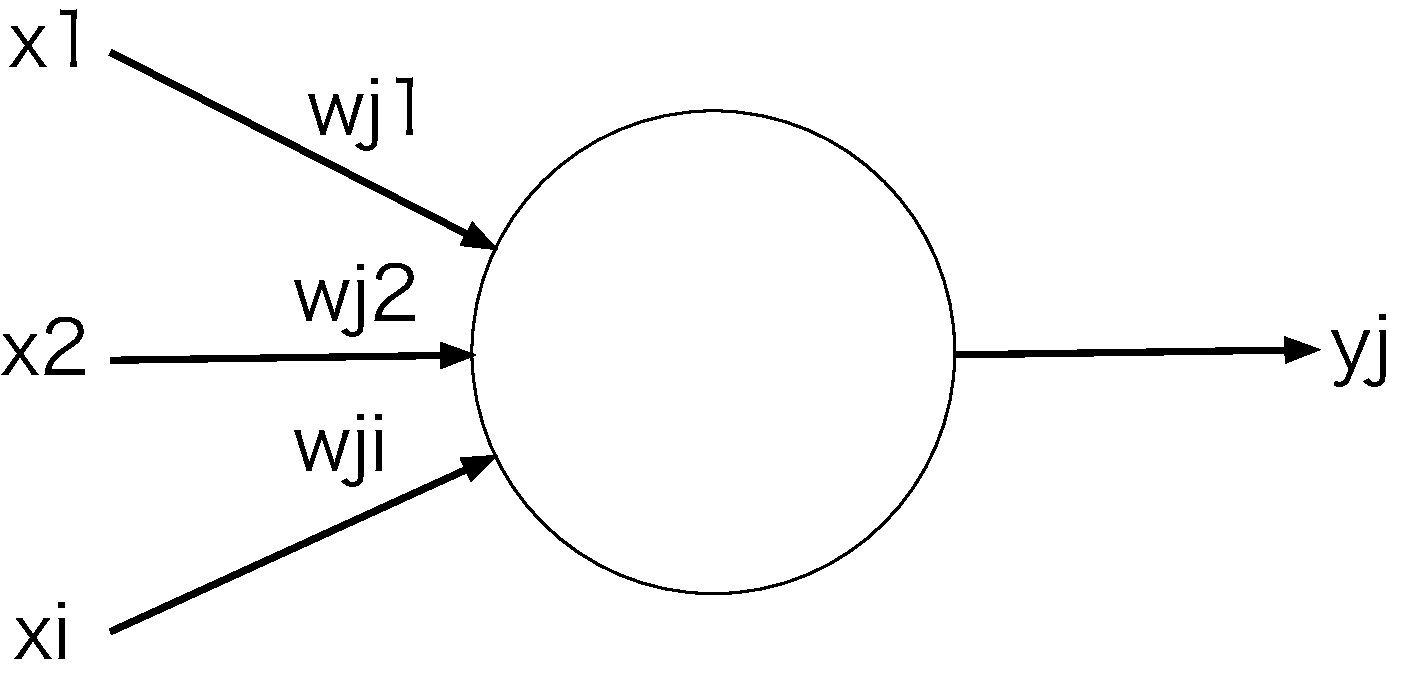
\includegraphics[bb=0 0 683 330, width=6cm]{Figures/neuron.pdf}
  \caption{ニューラルネットワークにおけるニューロン}
  \label{neuron}
\end{figure}

\begin{equation}
\label{calc-neuron}
y_j = f(\sum_i w_{ji} x_i + b_j).
\end{equation}

ただし,ただニューラルネットワークを構築して入力を与えただけでは,期待した出力が得られることは稀である.
そのため,期待した出力が得られるように誤差逆伝播法を用いて結合荷重とバイアスを更新していく,ニューロンの学習を行わなければならない.
学習を行うためには,何を目標に結合荷重やバイアスを更新していくのかという基準を設定する必要がある.
これは損失関数と呼ばれ,ニューラルネットワークにより得られた出力が,期待する出力(以下,教師信号)とどれだけの誤差があるかを定量的に測るために用いられる.

ニューロンの学習を行う際は,図\ref{bp}のような縦軸に損失関数(エネルギー関数)$E$,横軸に結合荷重$w$を置いたグラフで,$E$を最小化するような$opt\_w$に近づくように結合荷重を更新していく(勾配法).

\begin{figure}[hbtp]↲
    \centering↲
    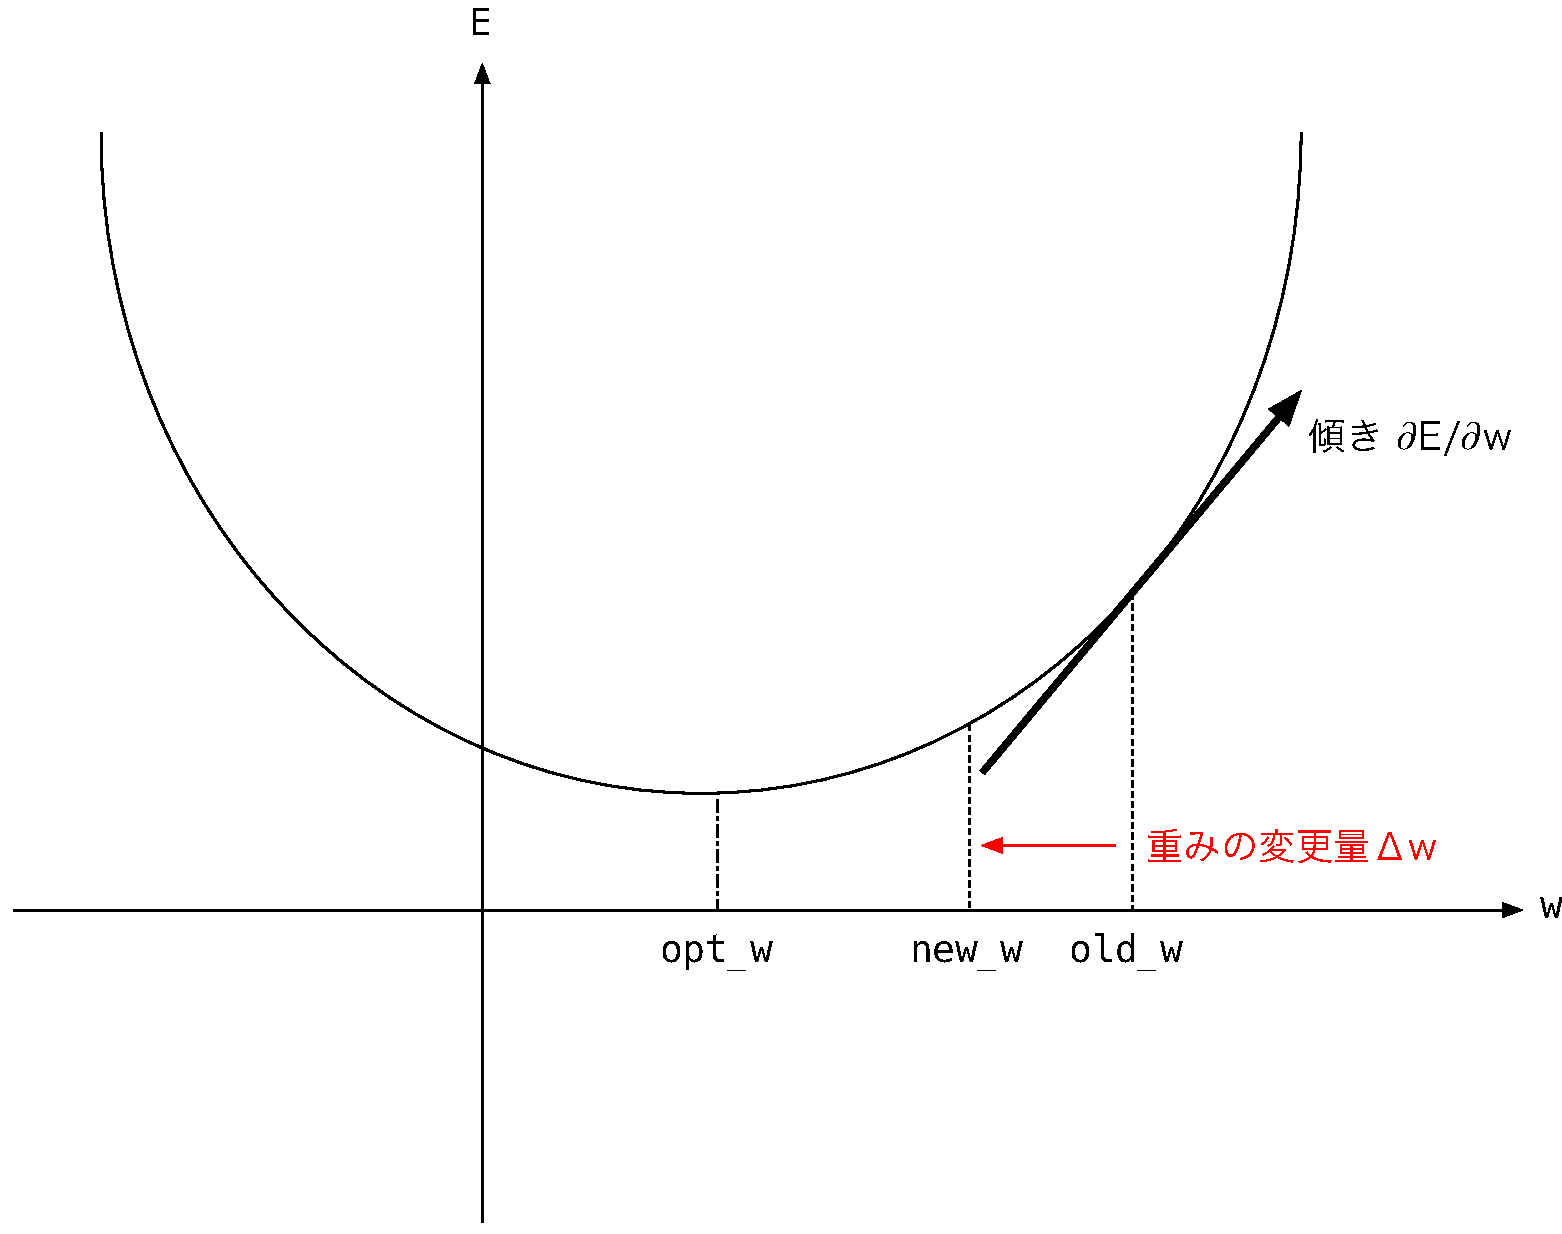
\includegraphics[bb=0 0 749 592, width=9cm]{Figures/bp.pdf}↲
    \caption{ニューロンの結合荷重の更新}↲
    \label{bp}↲
\end{figure}↲

更新した$new\_w$は,式\ref{w-new}で得られる.
\begin{equation}↲
\label{w-new}↲
new\_w = old\_w + \Delta w.↲
\end{equation}↲

式\ref{w-new}における$\Delta w$が結合荷重の変更量となるのだが,これは式\ref{delta-w}で得られる.
\begin{equation}↲
\label{delta-w}↲
\Delta w = - \eta \frac{\partial E}{\partial w}.↲
\end{equation}↲

$\eta$は学習率を表し,どれだけの割合で結合荷重を更新するかを示している.
この値を小さくすることで,結合荷重の更新幅が小さくなる.
その後ろの$\frac{\partial E}{\partial w}$は傾きを示す.↲
結合荷重$w$が$opt\_w$に近づくためには,傾きが正の場合は$\Delta w$が負に,傾きが負の場合は$\Delta w$が正になる必要がある.↲
そのため,$\eta \frac{\partial E}{\partial w}$の結果得られた値の符号を逆にしている.↲

結合荷重の変更量$\Delta w$を得るために必要な傾き$\frac{\partial E}{\partial w}$は,式\ref{ew}で得られる.
\begin{equation}↲
\label{ew}↲
\frac{\partial E_n}{\partial w_{ji}} = \frac{\partial E_n}{\partial a_j} \frac{\partial a_j}{\partial w_{ji}} = \frac{\partial E_n}{\partial a_j} x_i.↲
\end{equation}↲
↲
式\ref{ew}は,合成関数の微分の公式を用いて式変形を行っている.↲
$x_i$は学習中のニューロンに入力された値を示している.↲
ここで,$\frac{\partial E_n}{\partial a_j}$を$\delta_j$と置く.↲
この$\delta_j$と学習中のニューロンの入力値$x_i$を掛けることで傾きが得られ,これに$- \eta$を掛けることで結合荷重の変更量$\Delta w$が得られる.

前述したように,損失関数を用いて教師信号との誤差を測るために用いるのは出力層の出力値である.
ここで,出力層ニューロンの活性化関数と損失関数が特定の組み合わせであれば,$\delta_j$は式\ref{easy-delta}で得られる.
\begin{equation}↲
\label{easy-delta}↲
\delta_j = y_j - t_j.↲
\end{equation}↲

式\ref{easy-delta}における$y_j$は出力層より得られた出力値,$t_j$は教師信号である.
このように極めて単純な計算式で$\delta_j$を得られるため,基本的に出力層では損失関数と活性化関数を合わせて考えるのが一般的である.

まず,ニューラルネットワークで回帰を行う場合は,活性化関数と損失関数にそれぞれ恒等写像(式\ref{identity})と最小二乗誤差(式\ref{lsm})を用いる.
\begin{equation}↲
\label{identity}↲
f(a_j) = a_j.↲
\end{equation}↲
↲
\begin{equation}↲
\label{lsm}↲
E_n = \frac{1}{2} \sum_{k=1}^K (y_{nk} - t_{nk})^2.↲
\end{equation}↲

ニューラルネットワークで二値分類を行う場合は,活性化関数と損失関数にそれぞれシグモイド関数(式\ref{sigmoid})と交差エントロピー誤差(式\ref{ce-1})を用いる.
\begin{equation}↲
\label{sigmoid}↲
f(a_j) = \frac{1}{1 + e^{-a_j}}.↲
\end{equation}↲
↲
\begin{equation}↲
\label{ce-1}↲
E_n = - \sum_{k=1}^K \{t_{nk} \ln y_{nk} + (1 - t_{nk}) \ln (1 - y_{nk)}\}.↲
\end{equation}↲

また,ニューラルネットワークで多クラス分類を行う場合は,活性化関数と損失関数にそれぞれソフトマックス関数(式\ref{softmax})と交差エントロピー誤差(式\ref{ce-2})を用いる.
\begin{equation}↲
\label{softmax}↲
f(a_j) = \frac{e^{a_j}}{\sum_{k=1}^K e^{a_k}}.↲
\end{equation}↲
↲
\begin{equation}↲
\label{ce-2}↲
E_n = - \sum_{k=1}^K t_{nk} \ln y_{nk}.↲
\end{equation}↲

このような組み合わせで出力層を構築することで,前述した式\ref{easy-delta}で$\delta_j$を得られる.

ニューラルネットワークが入力層を含めて3層以上あるような複雑なもので中間層を学習したい場合,この$\delta_j$は式\ref{delta-2}で得られる.
\begin{equation}↲
\label{delta-2}↲
\delta_j = \frac{\partial f}{\partial a_j} \sum_{k=1}^K w_{kj} \delta_k.↲
\end{equation}↲

つまり,学習しているニューロンの活性化関数を微分したものと,出力層に一つ近い層の各結合荷重と$\delta$を掛けたものの総和を掛けることで,中間層の$\delta_j$が得られる.

以上で学習に必要な傾きが得られるが,これを用いた結合荷重の更新方法として式(\ref{w-new})を改良したアルゴリズムが複数考案されている.

まず,確率的勾配降下(SGD)というものがある(式\ref{sgd}).
\begin{equation}↲
\label{sgd}↲
new\_w_{ji} = old\_w_{ji} - \eta \delta_j x_i - \eta \lambda old\_w_{ji}.↲
\end{equation}↲
↲
$- \eta \lambda old\_w_{ji}$は荷重減衰と呼ばれるもので,$\lambda$を正の小さな定数に設定することで傾きがゼロの場合でも結合荷重を減らすことができるというものである.↲
$\eta$の値が結合荷重の更新に強く影響するため,通常は学習の初期段階では大きめの値にし,学習が進むにつれて小さくしていく.↲

次に,AdaGrad\cite{3-adagrad}というものがある(式\ref{adagrad}).↲
\begin{eqnarray}↲
\label{adagrad}↲
new\_g_{ji} = old\_g_{ji} + (\delta_j x_i)^2. \nonumber \\↲
new\_w_{ji} = old\_w_{ji} - \frac{\eta}{\sqrt{new\_g_{ji} + \epsilon}} \delta_j x_i.↲
\end{eqnarray}↲
↲
これは,過去の傾きの二乗和を結合荷重ごとに覚えておき($new\_g_{ji}$),その平方根で$\eta$を割ったものを学習率とする.↲
これにより,総更新量が少ない結合荷重はより大きな幅で,総更新量が多い結合荷重はより小さな幅で更新がなされる.↲
この方式では,学習率が自動的に調整される\cite{3-adagrad-detail}.↲

また,Adam\cite{3-adam}というものがある(式\ref{adam}).
\begin{eqnarray}
\label{adam}
new\_m = \beta_1 old\_m + (1 - \beta_1) \delta_j x_i.\nonumber \\
new\_\nu = \beta_2 old\_\nu + (1 - \beta_2) (\delta_j x_i)^2.\nonumber \\
new\_\hat{m} = \frac{new\_m}{1 - \beta^t_1}.\nonumber \\
new\_\hat{\nu} = \frac{new\_\nu}{1 - \beta^t_2}.\nonumber \\
new\_w_{ji} = old\_w_{ji} - \frac{\alpha}{\sqrt{new\_\hat{\nu}} + \epsilon} new\_\hat{m}.
\end{eqnarray}
↲
まず,傾きの一次モーメント(平均値)と二次モーメント(分散した平方偏差)の概算値を求める($new\_m$及び$new\_\nu$).
そしてこれらの偏りをバイアス補正した推定値を計算することで小さくし($new\_\hat{m}$及び$new\_\hat{\nu}$),これらを用いて結合荷重の更新を行う\cite{3-adam-detail}.

他にも様々なアルゴリズムが提案されている.↲

\section{Autoencoder}
Autoencoderとは,図\ref{autoencoder}のような入力層と出力層のニューロン数を入力データの次元数と同数にし,中間層のニューロン数を一定の割合で削減した3層構造のニューラルネットワークにおいて,入力データと教師信号に同じデータを用いて教師あり学習させたものである.
入力層から中間層への処理をエンコーダ,中間層から出力層への処理をデコーダと呼ぶ.
中間層と出力層の活性化関数は自由に選ぶことができるが,出力層の出力値が教師信号を表現できるような活性化関数を選ばなければならない.

\begin{figure}[hbtp]
  \centering
  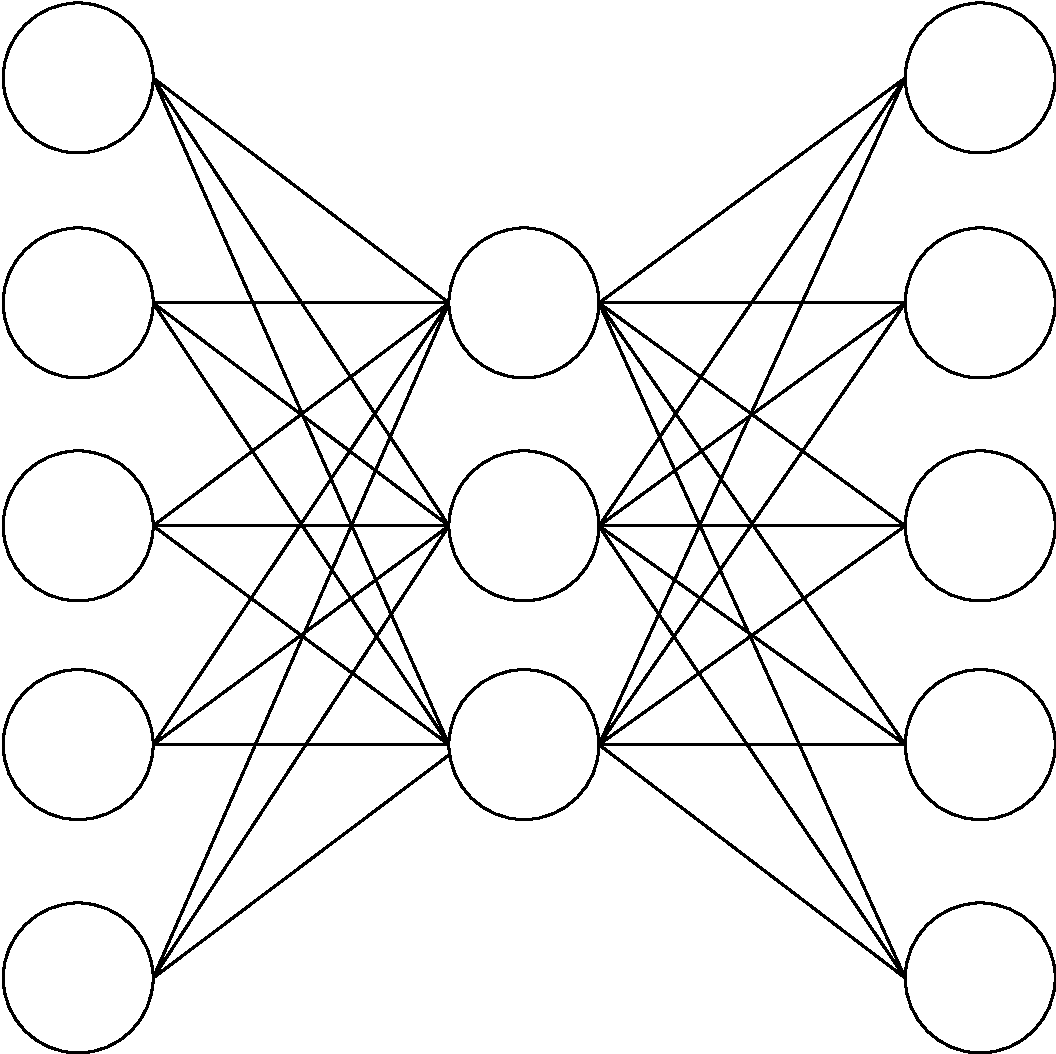
\includegraphics[bb=0 0 507 506, width=6cm]{Figures/autoencoder.pdf}
  \caption{Autoencoder}
  \label{autoencoder}
\end{figure}

Autoencoderの学習を進めた結果出力層の出力と教師信号との誤差が無くなった場合,中間層においてより少ないニューロン数で入力データの情報を表現できていると見ることができる.
このことから,学習済みのAutoencoderからデコーダの部分を取り除き,エンコーダの出力を別のニューラルネットワークへの入力値として渡すことで,入力データの特徴抽出器として用いることができる.

\section{Denoising Autoencoder}
Denoising Autoencoderとは,Autoencoderで用いる入力データに対し一定の割合でランダムなノイズを付与し,ノイズを付与する前の元データを教師信号として与えて教師あり学習させたものである.
入力データにランダムなノイズを付与して学習させることで,入力データの特徴を抽出することに加えてノイズの除去についても学習しなければならなくなり,ノイズに強くより汎化能力の高い特徴抽出器となる.

ノイズの付与方法として,入力データのうちランダムに選択したデータを0にするマスキングノイズや,0か1にする胡麻塩ノイズなど様々なものがある.

\section{Dropout}
Dropoutとは,図\ref{dropout}のように一定の割合でランダムに一部のニューロンを無視して学習を行うものである.
学習後のニューラルネットワークで推定を行う際は,各ニューロンの出力値にDropoutした割合を掛ける.

ニューラルネットワークの学習時にランダムで一部のニューロンを無視することから,複数の独立したニューラルネットワークを学習しているとみなすことができる.
そして推定時にはそれらニューラルネットワークから得られた出力の平均値を求めていると考えられるため,汎化能力がより高くなる.

\begin{figure}[hbtp]
  \centering
  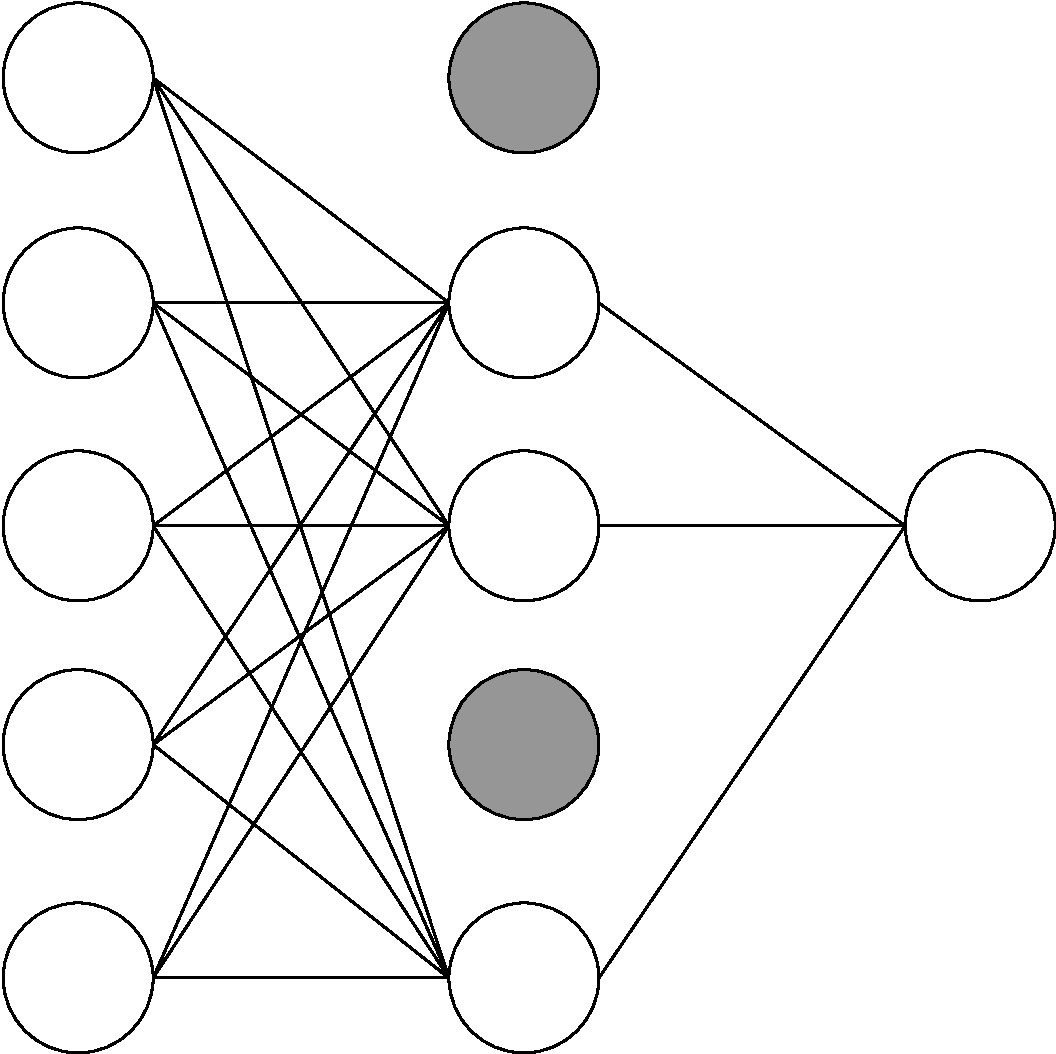
\includegraphics[bb=0 0 507 506, width=6cm]{Figures/dropout.pdf}
  \caption{Dropout}
  \label{dropout}
\end{figure}

% @suppress WordNumber
\section{モーションデータの取得}
本システムは,モーションデータの取得にAndroid端末で一般的に搭載されている加速度センサ(TYPE\_LINEAR\_ACCELERATION)と角速度センサ(TYPE\_GYROSCOPE)を用いる.
モーションセンサの座標系は図\ref{sensor}のようになっており,直線で示した方向に端末を動かすことで正の加速度が得られ,曲線で示した方向に端末を回転させることで正の角速度が得られる\cite{3-sensor-coordinate}.
センサ登録時に指定できるモーションデータの取得間隔はSENSOR\_DELAY\_FASTESTを指定しており,研究で使用したLGエレクトロニクス社とGoogle社によって開発されたNexus 5では,およそ5ミリ秒間隔でモーションデータが取得されていることを確認した.
ただし,SENSOR\_DELAY\_FASTESTなどによる取得間隔の指定はあくまでシステムへのヒントであり,システムによって変動する可能性がある\cite{3-sensor-delay}.

\begin{figure}[hbtp]
  \centering
  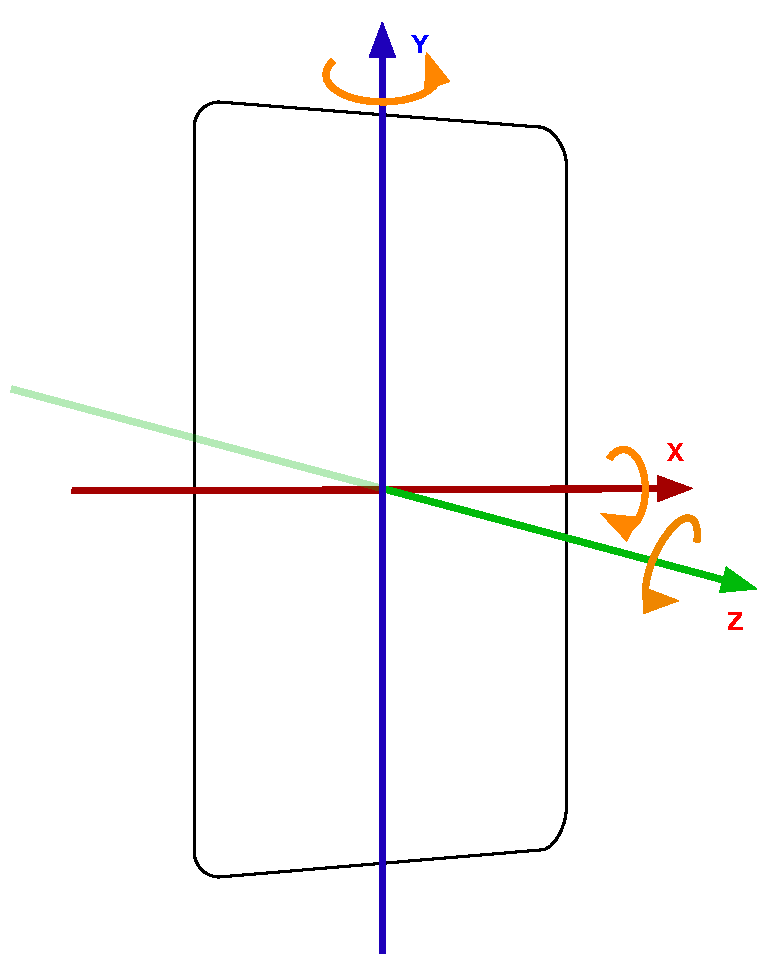
\includegraphics[bb=0 0 372 469, width=6cm]{Figures/sensor.pdf}
  \caption{モーションセンサの座標系}
  \label{sensor}
\end{figure}

\chapter{提案システム}
本章では,本研究で開発したスマートフォンのモーションセンサを利用した個人認証システムについて説明する.

\section{システムの概要}
本システムは,Android端末に一般的に搭載されている加速度センサと角速度センサを用いてモーションデータを収集し,Denoising Autoencoderとその後ろに識別用ニューロンを繋げた識別器を用いて個人認証を行う.
本システムには,登録モードと認証モードという二つの動作モードがある.
登録モードでは,入力されたモーションデータの一部を平均が0で分散が1のガウシアンノイズを用いて上書きしたものを用いて,Denoising Autoencoderで特徴を学習させる.
その後識別用ニューロンを繋いで入力データに対する教師信号として0.0を,入力データと同じ値域・次元数で生成した乱数でデータの一部を上書きしたダミーデータに対する教師信号として1.0を与えて識別器の学習を行う.
認証モードでは,入力されたモーションデータを学習済みの識別器に入力し,得られた出力を用いて個人認証を行う.

\subsection{動作モード選択}
Androidアプリケーションを起動すると,図\ref{start}のスタート画面が表示される.
画面下部にある``Start''ボタンを押すことで,図\ref{select-mode}の動作モード選択ダイアログが表示される.
``Registration''を選択すると登録モードに,``Authentication''を選択すると認証モードに遷移する.

% @suppress DuplicatedSection
\subsection{登録モード}
登録モードに遷移すると,図\ref{reg-input-name}のユーザ名入力画面が表示される.
ここでは登録するユーザ名を入力する.
ユーザ名を入力して画面下部にある``OK''ボタンを押すことでユーザ名が正しく入力されたか確認する処理が行われ,確認できれば図\ref{registration}のモーション入力画面が表示される.
ユーザ名が入力されていない,もしくは空白文字しか入力されていない場合は図\ref{reg-input-name-toast}のようにAndroidシステムに標準で用意されている通知機能であるToastを用いてユーザにエラーを通知する.

モーション入力画面では,画面下部の``モーションデータ取得''ボタンを押している間,加速度センサと角速度センサそれぞれにデータを取得するための専用スレッドが起動して各センサからデータが取得・蓄積される.
また,データ取得用スレッドの起動と同時に時間計測用スレッドも起動し,1秒経過毎に端末をバイブレートさせることでユーザにモーション入力の経過時間を伝える.
モーション入力中に任意のタイミングで``モーションデータ取得''ボタンから指を離すことで,モーション入力を終了できる.
モーション入力はデフォルトでは3回となっているが,画面右上のハンバーガーメニュー,もしくは端末に搭載されたメニューボタンを押すことで表示される図\ref{reg-menu}のメニュー画面から,``データ取得回数設定''を選択することで回数を変更できる.
``データ取得回数設定''を選択すると,図\ref{reg-change-time}のダイアログが表示される.
画面上にあるスライダーを操作して左右に動かすことで,データ取得回数を増減でき,画面下部の``OK''ボタンを押すことで設定が反映される.
また,先ほどのメニュー画面から``リセット''を選択すると,図\ref{reg-reset}のダイアログが表示される.
ここで``YES''を選択することで,モーションデータの取得状態をリセットし,一からモーション入力をやり直すことができる.

モーション入力が終わるたびに,取得したモーションデータのデータ数が確認される.
加速度センサ及び角速度センサから得られたX軸データのいずれかのデータ数が10個を下回っていた場合,図\ref{reg-recollect}のダイアログを表示し,ユーザに再度モーションを入力させる.
設定回数分のモーション入力が終わると図\ref{reg-progress}のプログレスダイアログが表示され,後述するモーションデータの加工及び識別器の学習を行うスレッドが起動する.

モーションデータの加工及び識別器の学習が終わると図\ref{reg-finish}のダイアログが表示される.
``OK''ボタンを押すことでユーザ名と暗号化した学習済み識別器のパラメータ,データの次元数を他アプリからの読み書きができない形で端末に保存し,スタート画面に遷移する.
何らかの原因で識別器の学習ができなかった場合は図\ref{reg-error}のダイアログが表示される.
``OK''ボタンを押すことでモーションデータの取得状態がリセットされるので再度モーションを入力する.

% @suppress DuplicatedSection
\subsection{認証モード}
認証モードに遷移すると,図\ref{auth-input-name}のユーザ名入力画面が表示される.
ここでは認証するユーザ名を入力する.
ユーザ名を入力して画面下部にある``OK''ボタンを押すことで登録モードで保存されたユーザ名のリストから入力されたユーザ名と合致するものが存在するか検索され,存在していた場合は図\ref{authentication}のモーション入力画面が表示される.
存在していなかった場合は,図\ref{auth-input-name-toast}のようにToastを用いてユーザにエラーを通知する.

モーション入力画面では,画面下部の``モーションデータ取得''ボタンを押している間,加速度センサと角速度センサそれぞれにデータを取得するための専用スレッドが起動して各センサからデータが取得・蓄積される.
また,データ取得用スレッドの起動と同時に時間計測用スレッドも起動し,1秒経過毎に端末をバイブレートさせることでユーザにモーション入力の経過時間を伝える.
モーション入力中に任意のタイミングで``モーションデータ取得''ボタンから指を離すことで,モーション入力を終了できる.
モーション入力は1回となっており,登録モードと違い変更はできない.

モーション入力が終わると,取得したモーションデータのデータ数が確認される.
加速度センサ及び角速度センサから得られたX軸データのいずれかのデータ数が10個を下回っていた場合,図\ref{auth-recollect}のダイアログを表示し,ユーザに再度モーションを入力させる.
設定回数分のモーション入力が終わると図\ref{auth-progress}のプログレスダイアログが表示され,後述するモーションデータの加工及び識別器による個人認証を行うスレッドが起動する.

モーションデータの加工及び個人認証が終わると,認証結果をダイアログで表示する.
認証に成功すれば図\ref{auth-succeed}のダイアログが表示され,``OK''ボタンを押すことでスタート画面に遷移する.
認証に失敗すれば図\ref{auth-failure}のダイアログが表示され,``OK''ボタンを押すことでモーションデータの取得状態がリセットされ,再度個人認証を行える.

\section{モーションデータの加工}
登録モードと認証モードのいずれも,モーションセンサから得られたデータはニューラルネットワークで用いる前に,``データ数の均一化''・``フーリエ変換を用いたローパスフィルタ''・``角速度から変位,角速度から角度への変換''・``変位データを角度データで回転''という四つの加工を行う.

\subsection{データ数の均一化}
本システムでは,モーション入力を任意の時間で行える.
この際,登録モードにおけるデフォルトでは3回のモーション入力によるモーションデータ,認証モードでは登録時に用いたモーションデータと新たに入力されたモーションデータ間でデータ数の差異が生じる場合がある.
本システムで用いたニューラルネットワークでは入力されるデータにおける次元数のばらつきは許容できないため,事前にデータ数を均一化する必要がある.

登録モードでは,最も入力時間の長かったデータを基準に他のデータに対して末尾にゼロを補填する方法を用いる.
認証モードでは,登録時に用いたデータの長さを基準に新たに入力されたデータが短い場合は末尾にゼロを補填し,長い場合は末尾を切り落とす方法でデータ数を均一化している.

% @suppress ParagraphNumber InvalidSymbol
\subsection{ローパスフィルタ}
モーションを入力している際に生じる手の震えなどによるモーションデータへの影響を抑えるために,フーリエ変換を用いたローパスフィルタ処理を実装している.
時間軸領域で表されるデータをフーリエ変換を用いて周波数領域に変換すると,モーション入力中に生じた手の震えなどによるデータが高周波成分として現れる.
この高周波成分を取り除いた上で元の時間軸領域で表されるデータに逆変換するローパスフィルタ処理を行うことで,手の震えなどによる影響の少ないデータを得られる.

フーリエ変換の実装には,CERNのColt Project\cite{4-colt-project}で開発された科学技術計算用ライブラリであるColtをマルチスレッド化したParallel Colt\cite{4-parallel-colt}に含まれている,JTransforms\cite{4-jtransforms}を用いた.

この処理をソースコード\ref{source-lowpass}に示す.

\lstinputlisting[caption=ローパスフィルタ, label=source-lowpass, style=MyJava]{Code/lowpass.java}

% ローパスフィルタの比較グラフ
ローパスフィルタ処理によるデータの変化を示したグラフを図\ref{graph-lowpass}に示す.

\begin{figure}[hbtp]
  \centering
  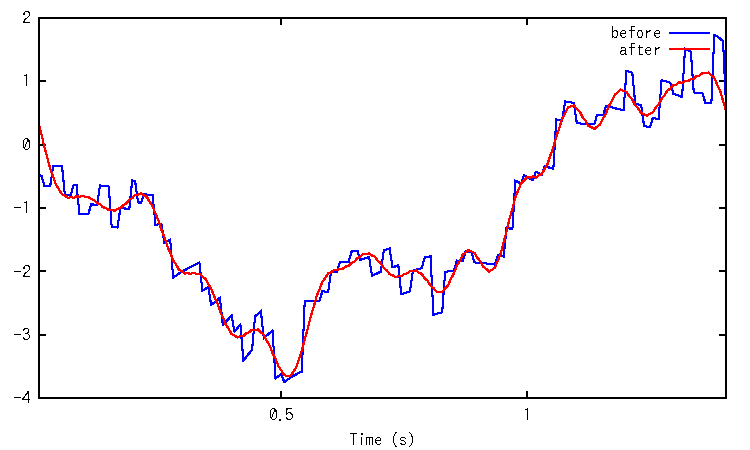
\includegraphics[bb=0 0 360 216, width=12cm]{Graphs/lowpass.pdf}
  \caption{ローパスフィルタ処理によるデータの変化}
  \label{graph-lowpass}
\end{figure}

青色で示した線がローパスフィルタ処理前のグラフ,赤色で示した線が処理後のグラフである.

% @suppress ParagraphNumber InvalidSymbol
\subsection{加速度から変位,角速度から角度への変換}
% ドリフトの影響があるため,足し合わせていく処理はしない
ローパスフィルタ処理したデータに対して,次に加速度から変位,角速度から角度に変換する処理を行う.
加速度から変位への変換は式\ref{accel-to-displacement}で行う.
\begin{equation}
\label{accel-to-displacement}
x = \frac{1}{2} a t^2.
\end{equation}

$x$は変位を,$a$は加速度を,$t$は加速度データの取得間隔を表している.
なお,本システムでは初速度を考慮しない.
この処理をソースコード\ref{source-accel-to-displacement}に示す.

\lstinputlisting[caption=加速度から変位への変換, label=source-accel-to-displacement, style=MyJava]{Code/accelToDisplacement.java}

また,角速度から角度への変換は式\ref{gyro-to-angle}で行う.
\begin{equation}
\label{gyro-to-angle}
y = g t.
\end{equation}

$y$は角度を,$g$は角速度を,$t$は角速度データの取得間隔を表している.
その処理をソースコード\ref{source-gyro-to-angle}に示す.

\lstinputlisting[caption=角速度から角度への変換, label=source-gyro-to-angle, style=MyJava]{Code/gyroToAngle.java}

% @suppress InvalidSymbol
\subsection{変位データを角度データで回転}
加速度から変位,角速度から角度へ変換したデータに対して,次は変位データを角度データで回転させる処理を行う.
この処理をソースコード\ref{source-rotate-vector}に示す.

\lstinputlisting[caption=変位データの角度データを用いた回転,合成, label=source-rotate-vector, style=MyJava]{Code/rotateVector.java}

変位データを回転させるcombineメソッドには,変位データの他にモーションデータ取得開始時点からどれだけ回転したかを保持するangleX・angleY・angleZのラジアンを渡している.
この際,各軸を中心に反時計回りで変位データを回転させるために,それぞれの正負を逆にした上でそのラジアンを求めている.

combineメソッドでは,渡されたラジアンについてそれぞれ$\sin$と$\cos$を求め,式\ref{rotate-matrix}の回転行列を用いてX軸・Y軸・Z軸の順に回転させている.

\begin{eqnarray}
\label{rotate-matrix}
R_x(\theta) = \left(
    \begin{array}{ccc}
        1 & 0 & 0 \\
        0 & \cos\theta & -\sin\theta \\
        0 & \sin\theta & \cos\theta
    \end{array}
\right). \nonumber \\
R_y(\theta) = \left(
    \begin{array}{ccc}
        \cos\theta & 0 & \sin\theta \\
        0 & 1 & 0 \\
        -\sin\theta & 0 & \cos\theta
    \end{array}
\right). \nonumber \\
R_z(\theta) = \left(
    \begin{array}{ccc}
        \cos\theta & -\sin\theta & 0 \\
        \sin\theta & \cos\theta & 0 \\
        0 & 0 & 1
    \end{array}
\right).
\end{eqnarray}

\section{ニューラルネットワークによる学習と識別}
本システムは,図\ref{system-nn}のようなDenoising Autoencoderと識別用ニューロンを繋げたニューラルネットワークにより個人認証を行う.


\begin{figure}[hbtp]
  \centering
  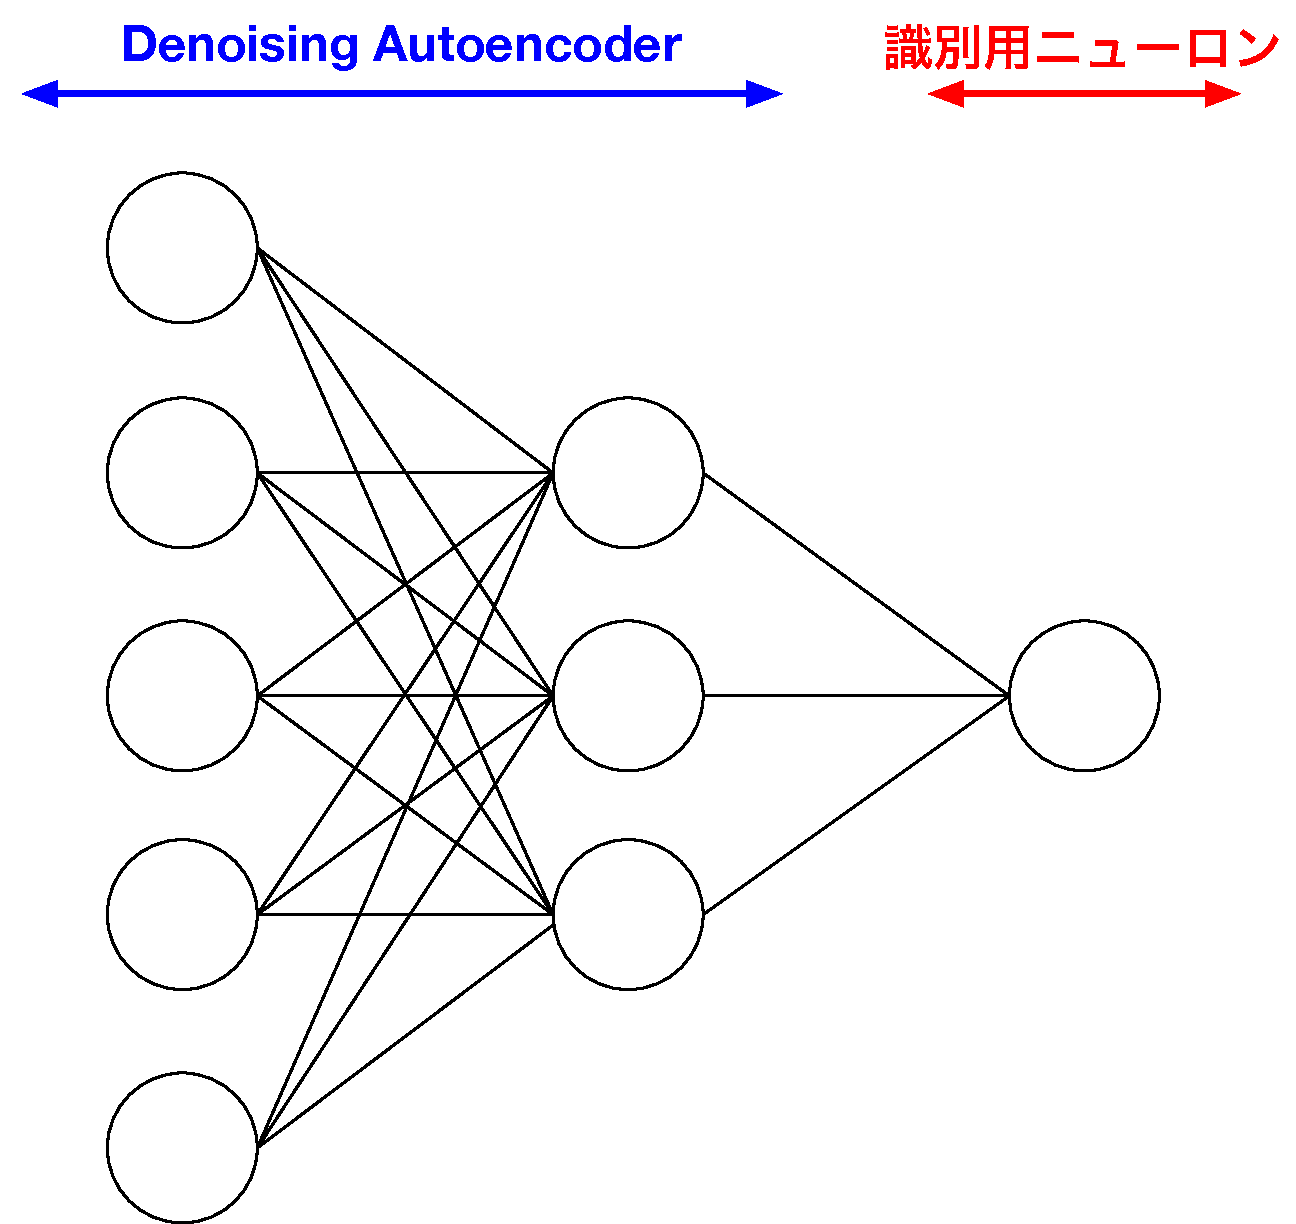
\includegraphics[bb=0 0 622 587, width=9cm]{Figures/system-nn.pdf}
  \caption{識別に用いるニューラルネットワーク}
  \label{system-nn}
\end{figure}

本システムでは,基本的にNVIDIA製GPUを搭載しCUDA\cite{4-cuda}を利用したGPGPUによる高速演算が可能な計算機上で動作するプログラム(以下,サーバ)でニューラルネットワークに関する処理を実行する.
Android端末上で動作するプログラム(以下,クライアント)とサーバでデータをやりとりする際にはTCPソケットを用いる.

% @suppress ParagraphNumber DuplicatedSection InvalidSymbol JapaneseNumberExpression JapaneseAmbiguousNounConjunction
\subsection{登録モード}
登録モードでは,動作モード値・ユーザ名・前述の加工を行ったモーションデータをTCPソケットを用いてサーバに送信する.
サーバ側ではこれらデータをJavaで書かれたプログラムで受信し,JNI\cite{4-jni}を用いてC++で書かれたニューラルネットワークプログラムに処理を移す.

ニューラルネットワークプログラムでは,まずDenoising Autoencoderの学習を行う.
%入力データにノイズをのせて学習
まず,受け取ったモーションデータを平均が0,分散が1になるように正規化する.
この処理をソースコード\ref{source-normalize}に示す.

\lstinputlisting[caption=モーションデータの正規化処理, label=source-normalize, style=MyCpp]{Code/normalize.cpp}

そして,正規化した各モーションデータのそれぞれ30\%に,平均が0で分散が1のガウシアンノイズによるノイズ加工を行う.
この処理をソースコード\ref{source-dA-noise}に示す.

\lstinputlisting[caption=dA学習時のノイズ加工, label=source-dA-noise, style=MyCpp]{Code/dA-noise.cpp}

ノイズ加工を行った後,中間層のニューロン数を入力層や出力層のニューロン数から50\%削減し,中間層の活性化関数にシグモイド関数,出力層の活性化関数に恒等関数を用いたDenoising Autoencoderを構築する.
訓練データにノイズ加工を行ったモーションデータを,教師信号にノイズ加工を行う前のモーションデータを与え,損失関数に最小二乗誤差を用いて300回の学習を行う.
また,訓練時に中間層ニューロンのうち50\%をランダムにDropoutさせる.

%学習が完了したら,次は識別用ニューロンをつないで,ダミーデータを生成して学習する
Denoising Autoencoderの学習が終われば,Denoising Autoencoderのパラメータを固定して,この後ろに活性化関数にシグモイド関数を用いたニューロンを繋げる.
そして,正規化する前のモーションデータの値域で生成したランダム値でデータの20\%を上書きしたダミーデータを生成し,正規化する.
%こちらもDropout率や学習回数などを
訓練データに正規化したモーションデータとダミーデータを,教師信号にそれぞれ0.0と1.0を与え,損失関数に交差エントロピー誤差を用いて誤差が0.1未満になるまで最大1000回の学習を行う.
この際Dropoutを無効にし,Denoising Autoencoderの出力に対して1から先ほどの学習時に適用したDropout率を引いた0.5を掛ける.

%学習できたら,学習済みニューラルネットワークのパラメータをAndroid端末側に送り返す
学習が終われば,ニューラルネットワークにおける各層ごとのニューロンが持つパラメータを文字列として連結したデータをクライアントに送る.

%Android端末側でうけとって,保存してetc
クライアント側はこのデータを受け取り,暗号化した上で他アプリからの読み書きができない形で保存する.

% @suppress DuplicatedSection
\subsection{認証モード}
認証モードでは,動作モード値・ユーザ名・前述の加工を行ったモーションデータ・登録モードにおいて保存した学習済みニューラルネットワークのパラメータをTCPソケットを用いてサーバに送信する.
サーバ側ではこれらデータをJavaで書かれたプログラムで受信し,JNIを用いてC++で書かれたニューラルネットワークプログラムに処理を移す.

ニューラルネットワークプログラムでは,まず受け取ったモーションデータを平均が0,分散が1になるように正規化する.
次に,受け取った学習済みニューラルネットワークのパラメータをもとにニューラルネットワークを構築する.
構築できたらこれに正規化したモーションデータを与え,出力値を得る.
そして,得られた出力値をクライアントに送る.

クライアント側はこの値を受け取り,値が0.2未満であれば認証成功とし,0.3以上であれば認証失敗とする.

また,認証モードに限り,端末が何らかの理由でサーバに接続できない場合は端末のローカルでサーバと同等の処理が行えるようにしている.

\chapter{評価}
本章では,本研究で開発した個人認証システムの識別精度と登録及び認証処理にかかる時間の評価を行う.

% @suppress ParagraphNumber JapaneseAmbiguousNounConjunction InvalidSymbol
\section{識別精度の評価}
認証精度の評価について,端末を持ち上げるモーションを対象とする.
本システムを用いてあらかじめ6名の被験者に端末を持ち上げるモーションを4回入力してもらい,モーションデータの収集を行った.
各被験者ごとに,モーションデータの最初の3回分を登録モードにおける学習データ,最後の1回分を認証モードにおける入力データとして識別器の学習と識別を10回ずつ試行した.
また,それぞれの試行時になりすまし認証データとして筆者自身が同様のモーションを入力して得たモーションデータも入力した.

\begin{table}[btph]
  \centering
  \caption{識別精度の評価結果}
  \label{auth-result}
  \begin{tabular}{|c|r|r|r|r|r|} \hline
    回数 & 1 & 2 & 3 & 4 & 5 \\ \hline
    A & 0.438653 & 0.314004 & 0.331712 & 0.189229 & 0.343942 \\
    なりすまし & 0.999996 & 1 & 1 & 1 & 1 \\ \hline
    B & 0.643093 & 0.486959 & 0.30173 & 0.402533 & 0.333143 \\
    なりすまし & 0.92829 & 0.746492 & 0.471353 & 0.555157 & 0.990063 \\ \hline
    C & 0.463514 & 0.535742 & 0.429281 & 0.431916 & 0.660576 \\
    なりすまし & 0.511741 & 0.57337 & 0.585036 & 0.40849 & 0.897041 \\ \hline
    D & 0.542743 & 0.469785 & 0.478641 & 0.206191 & 0.316994 \\
    なりすまし & 0.51709 & 0.790494 & 0.860314 & 0.665402 & 0.366732 \\ \hline
    E & 0.369962 & 0.775177 & 0.930394 & 0.620721 & 0.861707 \\
    なりすまし & 0.425681 & 0.622781 & 0.823906 & 0.322503 & 0.808092 \\ \hline
    F & 0.427885 & 0.480025 & 0.526025 & 0.398201 & 0.602788 \\
    なりすまし & 0.440998 & 0.57856 & 0.40198 & 0.756612 & 0.580305 \\ \hline \hline
    回数 & 6 & 7 & 8 & 9 & 10 \\ \hline
    A & 0.451342 & 0.423822 & 0.25965 & 0.509021 & 0.202369 \\
    なりすまし & 1 & 1 & 1 & 1 & 0.997968 \\ \hline
    B & 0.335206 & 0.43043 & 0.403946 & 0.378164 & 0.412219 \\
    なりすまし & 0.605696 & 0.602051 & 0.312502 & 0.489541 & 0.951559 \\ \hline
    C & 0.416119 & 0.197132 & 0.515574 & 0.688828 & 0.635752 \\
    なりすまし & 0.612922 & 0.28289 & 0.712931 & 0.991952 & 0.580779 \\ \hline
    D & 0.403892 & 0.393019 & 0.457838 & 0.397036 & 0.63433 \\
    なりすまし & 0.677217 & 0.616272 & 0.60307 & 0.55076 & 0.533577 \\ \hline
    E & 0.558159 & 0.827285 & 0.816316 & 0.805877 & 0.741235 \\
    なりすまし & 0.457879 & 0.805894 & 0.486814 & 0.380957 & 0.529755 \\ \hline
    F & 0.403371 & 0.386153 & 0.492409 & 0.616016 & 0.389095 \\
    なりすまし & 0.430812 & 0.367287& 0.480061 & 0.511264 & 0.576477 \\ \hline
  \end{tabular}
\end{table}

この実験により識別器から得られた出力をまとめたものを表\ref{auth-result}に示す.
被験者Aと被験者Bについては本人のモーションデータから得られた出力が0に近く,なりすまし認証のモーションデータから得られた出力が1に近いことから良く識別できているといえる.
しかし他の4名の被験者について,なりすまし認証のモーションデータから得られた出力が本人のモーションデータから得られた出力より低く出ているものが多く,識別できていない結果となった.

本システムでは端末所有者のモーションデータとなりすまし認証によるモーションデータを識別するために,識別器の学習時に端末所有者のモーションデータのほかに,このデータと同じ値域で生成した乱数で一部を置き換えたダミーデータを用いた.
このダミーデータは元データの値域及び次元数に依存するため,端末所有者が入力したモーションが小さい場合は生成できる乱数の値域が限られることから,また次元数が少ない場合は置き換えるデータ数が少ないことから元データとの差があまり出ない可能性がある.
これにより,端末所有者が入力したモーションデータであってもなりすまし認証であると識別されてしまったのではないかと考えられる.

識別率の良かった被験者Aと良くなかった被験者Eのモーションデータを比較したものを図\ref{compare}に示す.

\begin{figure}[hbtp]
  \centering
  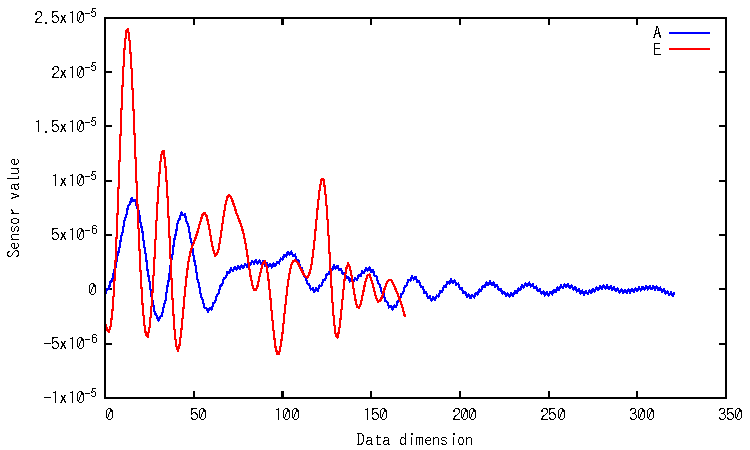
\includegraphics[bb=0 0 360 216, width=12cm]{Graphs/comp.pdf}
  \caption{被験者Aと被験者Eのモーションデータ比較}
  \label{compare}
\end{figure}

\section{登録及び認証の処理時間の評価}
本システムについて,登録及び認証の処理時間を計測した.
Androidのログ出力用APIとして用意されているLogクラス\cite{5-log}を用い,モーション入力が終了し計算処理中であることをユーザに示すプログレスダイアログが表示される部分と,登録及び認証処理が終わり処理結果が表示される前にプログレスダイアログが非表示となる部分にログ出力を行うコードを挿入した.
このログから出力される時刻情報から処理時間を求めて評価を行った.
また,認証モードについては端末内での計算処理も行えるため,こちらの処理時間も求めることとする.

評価の結果,サーバを用いた場合の登録処理ではおよそ65秒,認証処理ではおよそ2秒となった.
また,端末内での認証処理ではおよそ2.2秒となった.

ただし,モーションデータの次元数が多い場合や,サーバを多数のユーザが利用する場合はより長い処理時間を要すると考えられる.

% @suppress
\chapter{結論}
本研究では,一般的なスマートフォンに搭載されている加速度センサと角速度センサを利用し,端末を振る動きで個人認証を行うシステムを開発した.
そして,複数の被験者を対象にした認証精度の評価と登録及び認証の処理時間計測を行った.
認証精度の評価実験から,多くの被験者については本人のモーションデータとなりすまし認証によるモーションデータの識別がある程度明確にできたが,一部の被験者はなりすまし認証のデータで得られた識別器の出力がより低く出ており,上手く識別できていない.
また,本人のモーションデータとなりすまし認証によるモーションデータの識別ができた被験者についても,試行によっては識別できなくなるなどの不安定さが見られた.
本システムでは,端末所有者本人のモーションデータとなりすまし認証によるモーションデータを識別するために,端末所有者が入力したモーションデータの30\%を0で上書きしたダミーデータを用いた.
だが,端末所有者が入力したモーションデータに0に近い値が多く含まれる場合や,データの次元数が少なく上書きするデータ数が少なくなる場合は,端末所有者が入力したモーションデータとダミーデータの間の差が出ない可能性がある.
これによって,端末所有者が入力したモーションデータであってもなりすまし認証であると識別される場合があったのではないかと考えている.

また,本システムでは端末所有者が入力したモーションデータに0を上書きする際はランダムにデータを選択しているが,何らかの規則に従って0で上書きするかを決めることにより,識別器の不安定さを解消できる可能性がある.
加えて,ダミーデータの生成方法として0でデータを上書きする方法ではなく,何らかの別の方法を用いることができないかを検討する必要がある.

% また,望む機能を実現するためにどのような技術が他にあるか(畳み込みニューラルネットワークとか)
本システムではダミーデータを用いることで端末所有者のモーション入力を識別することを目指したが,畳み込みニューラルネットワークのようなより高度な人工ニューラルネットワークを用いて端末所有者の端末の振り癖を学習させることで,特定のモーションに縛られない自由度と精度の高い個人識別が実現できる可能性があるため,検討する必要がある.

\clearpage
\chapter*{謝辞}
本研究における個人認証システムの開発及び本稿の執筆にあたり,関西大学総合情報学部の小林孝史准教授,桑門秀典教授,堀井康史教授,田頭茂明教授に深く御礼申し上げます.
特に,小林孝史准教授には学部生の頃から毎週のゼミを中心に日頃から多くの御指導を賜り,御多忙の中時間を割いて下さったことに対し,心より感謝いたします.
また,小林研究室に所属する学部生と大学院生,先輩方,また総合情報学研究科で共に学んだ同輩の方々にも様々なご協力を頂きました.
特に,小林研究室に入り,研究テーマに悩んでいた際に先輩方からアドバイスを頂いたからこそ,この研究一筋で没頭することができました.
この場を借りて,御礼申し上げます.

また,大学院の講義でニューラルネットワークを教えて下さった林勲教授に対して,御礼を申し上げます.
講義を受けるまでニューラルネットワークの仕組みについてほぼ何も知らなかった私に対し,1から噛み砕いて,手を動かしつつ分かりやすく教えて下さったからこそ,本研究でもニューラルネットワークをシステムに組み込むことができました.


\begin{thebibliography}{10}
\renewcommand{\headrulewidth}{0pt}
\pagestyle{fancy}
\lhead{参考文献,参考URL等}
\chead{\empty}
\rhead{\thepage}
\lfoot{\empty}
\cfoot{\empty}
\rfoot{\empty}

\bibitem{1-smartphone}{総務省|電気通信サービスFAQ(よくある質問)|スマートフォンとはなんですか?,http://www.soumu.go.jp/main\_sosiki/joho\_tsusin/d\_faq/faq01.html,2017年1月27日確認.}
\bibitem{1-spread}{総務省,``平成28年版情報通信白書'',2016年.}

\end{thebibliography}

\clearpage
%\renewcommand{\headrulewidth}{0pt}
%\pagestyle{fancy}
%\lhead{付録}
%\chead{\empty}
%\rhead{\thepage}
%\lfoot{\empty}
%\cfoot{\empty}
%\rfoot{\empty}
\appendix

\chapter{提案システムの実装}
\lstinputlisting[caption=ローパスフィルタ, label=source-lowpass, style=MyJava]{Code/lowpass.java}

\lstinputlisting[caption=加速度から変位への変換, label=source-accel-to-displacement, style=MyJava]{Code/accelToDisplacement.java}

\lstinputlisting[caption=角速度から角度への変換, label=source-gyro-to-angle, style=MyJava]{Code/gyroToAngle.java}

\lstinputlisting[caption=変位データの角度データを用いた回転,合成, label=source-rotate-vector, style=MyJava]{Code/rotateVector.java}

\lstinputlisting[caption=モーションデータの正規化処理, label=source-normalize, style=MyCpp]{Code/normalize.cpp}

\lstinputlisting[caption=dA学習時のノイズ加工, label=source-dA-noise, style=MyCpp]{Code/dA-noise.cpp}

\chapter{識別器のパラメータ調整}
識別器のパラメータ調整における出力結果をまとめたものを以下に載せる.

\section{パラメータ変更に伴う被験者Aとなりすまし認証の出力}
\begin{longtable}[btph]{|c|c|r|r|r|r|r|}
  \centering
  \hline
    \multicolumn{1}{|c|}{ダミー割合} & \multicolumn{1}{c|}{入力} & \multicolumn{1}{c|}{10\%} & \multicolumn{1}{c|}{20\%} & \multicolumn{1}{c|}{30\%} & \multicolumn{1}{c|}{40\%} & \multicolumn{1}{c|}{50\%} \\ \hline \hline
    \multirow{2}{*}{0\%}  & 被験者 & 0.555086 & 0.304298 & 0.204448 & 0.363251 & 0.167029
         & なりすまし & 1 & 1 & 1 & 0.999999 & 1 \\ \cline{2-7} \\ \hline
    \multirow{2}{*}{10\%} & 被験者 & 0.564118 & 0.469948 & 0.610662 & 0.276341 & 0.252953
         & なりすまし & 1 & 1 & 0.999999 & 1 & 1 \\ \cline{2-7} \\ \hline
    \multirow{2}{*}{20\%} & 被験者 & 0.383344 & 0.692216 & 0.308345 & 0.327962 & 0.133113
         & なりすまし & 0.999995 & 1 & 0.999974 & 1 & 1 \\ \cline{2-7} \\ \hline
    \multirow{2}{*}{30\%} & 被験者 & 0.419408 & 0.699372 & 0.388538 & 0.163211 & 0.385198
         & なりすまし & 1 & 0.999687 & 0.999964 & 1 & 1 \\ \cline{2-7} \\ \hline
    \multirow{2}{*}{40\%} & 被験者 & 0.585243 & 0.170522 & 0.436479 & 0.362238 & 0.113613
         & なりすまし & 0.999999 & 1 & 1 & 1 & 1 \\ \cline{2-7} \\ \hline
    \multirow{2}{*}{50\%} & 被験者 & 0.530125 & 0.266473 & 0.326028 & 0.221857 & 0.156666
         & なりすまし & 1 & 1 & 1 & 1 & 1 \\ \cline{2-7} \\ \hline
    \multirow{2}{*}{60\%} & 被験者 & 0.53795  & 0.481888 & 0.527196 & 0.449104 & 0.156568
         & なりすまし & 0.999998 & 1 & 1 & 1 & 1 \\ \cline{2-7} \\ \hline
    \multirow{2}{*}{70\%} & 被験者 & 0.494861 & 0.43898  & 0.452982 & 0.238896 & 0.38547
         & なりすまし & 1 & 1 & 1 & 1 & 1 \\ \cline{2-7} \\ \hline
    \multirow{2}{*}{80\%} & 被験者 & 0.496032 & 0.322346 & 0.473375 & 0.34824  & 0.228593
         & なりすまし & 0.99999 & 1 & 0.999694 & 1 & 1 \\ \cline{2-7} \\ \hline
    \multirow{2}{*}{90\%} & 被験者 & 0.540851 & 0.725146 & 0.383797 & 0.504071 & 0.436995
         & なりすまし & 0.999352 & 0.999838 & 1 & 0.999951 & 1 \\ \cline{2-7} \\ \hline
    \multicolumn{1}{|c|}{ダミー割合} & \multicolumn{1}{c|}{入力} & \multicolumn{1}{c|}{60\%} & \multicolumn{1}{c|}{70\%} & \multicolumn{1}{c|}{80\%} & \multicolumn{1}{c|}{90\%} & \multicolumn{1}{c|}{} \\ \hline \hline
    \multirow{2}{*}{0\%}  & 被験者 & 0.0802036 & 0.122512  & 0.177721  & 0.0915504 &
         & なりすまし & 1 & 1 & 1 & 0.995389 & \\ \cline{2-7} \\ \hline
    \multirow{2}{*}{10\%} & 被験者 & 0.121232  & 0.103199  & 0.099126  & 0.123473  &
         & なりすまし & 1 & 1 & 1 & 1 & \\ \cline{2-7} \\ \hline
    \multirow{2}{*}{20\%} & 被験者 & 0.213511  & 0.0863974 & 0.0932137 & 0.0727035 &
         & なりすまし & 1 & 1 & 1 & 1 & \\ \cline{2-7} \\ \hline
    \multirow{2}{*}{30\%} & 被験者 & 0.764073  & 0.181448  & 0.118825  & 0.0811991 &
         & なりすまし & 0.999998 & 1 & 1 & 1 & \\ \cline{2-7} \\ \hline
    \multirow{2}{*}{40\%} & 被験者 & 0.0507103 & 0.131252  & 0.0834445 & 0.0709488 &
         & なりすまし & 1 & 1 & 0.999672 & 0.999988 & \\ \cline{2-7} \\ \hline
    \multirow{2}{*}{50\%} & 被験者 & 0.0838286 & 0.0685304 & 0.284507  & 0.122072  &
         & なりすまし & 0.992942 & 1 & 0.999994 & 0.999501 & \\ \cline{2-7} \\ \hline
    \multirow{2}{*}{60\%} & 被験者 & 0.186636  & 0.285555  & 0.208657  & 0.141091  &
         & なりすまし & 1 & 1 & 0.999987 & 0.999086 & 1 & \\ \cline{2-7} \\ \hline
    \multirow{2}{*}{70\%} & 被験者 & 0.142023  & 0.399493  & 0.17523   & 0.0676961 &
         & なりすまし & 1 & 0.999915 & 1 & 0.949006 & \\ \cline{2-7} \\ \hline
    \multirow{2}{*}{80\%} & 被験者 & 0.400451  & 0.229856  & 0.272355  & 0.13959   &
         & なりすまし & 0.999997 & 0.999905 & 0.993996 & 0.898188 & \\ \cline{2-7} \\ \hline
    \multirow{2}{*}{90\%} & 被験者 & 0.397789  & 0.462147  & 0.330115  & 0.282342  &
         & なりすまし & 1 & 0.998602 & 0.999743 & 0.957454 & \\ \cline{2-7} \\ \hline \hline
\end{longtable}


\end{document}
